\documentclass[%
a4paper,%
11pt,%
DIV12,%
BCOR20mm,%
twoside,%
openright,%
headsepline,%
bibtotocnumbered%
]{scrbook}

%%% Sprach-Konfiguration
\usepackage[utf8]{inputenc}
\usepackage[english]{babel}
\hyphenation{whe-ther}

%%% Grafik-Konfiguration
\usepackage{graphicx}
%\usepackage[hang]{subfigure}     % Subfigures if you need them
\usepackage{rotating}             % you can place sidewaysfigures with this!
\usepackage[format=hang]{caption} % Better-looking captions

%%% Schriftarten und Symbole
\usepackage[T1]{fontenc}

% -- Use this if you want some nicer fonts --
\usepackage{mathptmx}
\usepackage[scaled=0.9]{helvet}
% \usepackage{courier} % I don't like courier
\usepackage{ascii}

%\usepackage{latexsym}
%\usepackage[thickspace]{SIunits}

%%% Mathematik
\usepackage{amsmath}
\usepackage{amssymb}

%%% Sonstiges
\usepackage[below]{placeins} % Manages Floats
%\usepackage{calc}
\usepackage{ifthen}    % Needed for macros
%\usepackage{url}      % Typeset clicable URL's 
\usepackage{xspace}    % Useful for macros!
\usepackage{acronym}   % Acronym management package
\usepackage{blindtext} % Generates Lorem Ipsum for this template
\usepackage{booktabs}  % Typesets optimal tables; see documentation
%\usepackage{python}   % Python Scripting!

\usepackage{tikz}      % If you want to use TikZ for some figures
\usetikzlibrary{positioning}
\usetikzlibrary{automata}
\usetikzlibrary{arrows}
\usetikzlibrary{matrix}
\usetikzlibrary{fit}
\usetikzlibrary{calc}
\usetikzlibrary{chains}
\usetikzlibrary{patterns}
\usetikzlibrary{shadows}
\usetikzlibrary{shapes.geometric}
\usetikzlibrary{shapes.symbols}
\usetikzlibrary{shapes.arrows}
\usetikzlibrary{shapes.callouts}
\usetikzlibrary{decorations.shapes}
\usetikzlibrary{decorations.pathreplacing}
\usetikzlibrary{decorations.pathmorphing}

%%%% Define TikZ styles
%% Generic styles for pictures, nodes, ...
\tikzstyle{every picture}=[>=latex', double distance=2pt]
\tikzstyle{every node}=[font=\sffamily\small]

%% Utilities
\tikzstyle{reset}=[inner sep=1ex, minimum width=0mm, anchor=center]

%% Macros for MLA components
\tikzstyle{square}=[minimum width=8mm, minimum height=8mm]
\tikzstyle{component}=[draw, rectangle, rounded corners]
\tikzstyle{layer}=[component, drop shadow, fill=white]

%%%%% Setting up some layers
\pgfdeclarelayer{background}
\pgfdeclarelayer{foreground}
\pgfsetlayers{background,main,foreground}

  % See img/tikzsetup.tex for further explanations

%%% If you need code-listings
%\usepackage{listings}
%\lstloadlanguages{C}
%\lstset{%
%language=C,%
%basicstyle=\ttfamily\small,%
%keywordstyle=\bfseries,%
%identifierstyle=,%
%commentstyle=\itshape,%
%showstringspaces=false,%
%numbers=left,%
%numberstyle=\ttfamily\footnotesize,%
%numbersep=1em,%
%xleftmargin=12mm,%
%breaklines=true,%
%breakatwhitespace=true,%
%}

%%% Set up PDF-Stuff
%%% Set up hyperref if we are compiling with pdflatex
%%
\ifx\pdftexversion\undefined
\usepackage{hyperref}
\else
\usepackage[colorlinks=false,       %true => text des links wird farbig, false => farbiges kaestchen (wird nicht gedruckt) um schwarzen text
            linkcolor=black,        %nur bei colorlinks=true
            urlcolor=black,
            citecolor=black,
            bookmarks,                  % Bookmarks erstellen
            bookmarksopen=true,         % Bookmark beim Oeffnen anzeigen?
            pdfpagemode=UseOutlines,    % Bookmark beim Oeffnenanzeigen? (UseOutlines / none)
            bookmarksopenlevel=3,       % bis zu welcher Ebenen geoeffnet
            bookmarksnumbered,          % Kapitelnummern in Bookmarks
            pdftitle={see pdfsetup.tex on how to set a title here (and other pdf magic)},
            pdfsubject={Masterarbeit},
            pdfkeywords={input, some, keywords, here},
            pdfauthor={Input your name here!}
            ]{hyperref}
\fi

%%% 
%%
\ifx\pdftexversion\undefined
\else
\pdfoutput=1        % PDF-Ausgabe anschalten.
\pdfimageresolution=600
\pdfcompresslevel=9 % 0 keine kompression, 9 staerkste kompression
\fi

% vim: set ft=tex
  % Customize pdfsetup.tex

%%% Set up the Title
%%% Daten für die Titelseite. Bitte korrekt ausfüllen. ;-)
%%
\newcommand{\Title}{Writing a Masters Thesis using \LaTeXe and Advice from
Prof.\ John\ W.\ Chinneck}
\newcommand{\Type}{Masterarbeit}
\newcommand{\Author}{\href{mailto:mustermann@upb.de}{Manfred Mustermann}}
\newcommand{\Strasse}{Irgendeine Strasse 99}
\newcommand{\Matrikelnummer}{1234567}
\newcommand{\Ort}{33100 Paderborn}
\newcommand{\BetreuerA}{\href{mailto:holger.karl@upb.de}{Prof.\ Dr.\ Holger\ Karl}}
\newcommand{\BetreuerB}{\href{mailto:mitarbeiter@upb.de}{Mitarbeiter Sowieso}}
\newcommand{\Zweitgutachter}{\href{mailto:zweitgutachter@upb.de}{Prof.\ Dr.\ Sowieso Sowieso}}
\newcommand{\Date}{Abgabe-Datum hier eintragen}


%%% ------- DO NOT MODIFY BELOW HERE --------
%%
\newcommand{\Maketitle}{%
%
\titlehead{%
\includegraphics[scale=0.4]{img/uni-logo-woname}%
\hfill%
\raisebox{1em}{
\parbox[c]{10cm}{%
\begin{center}
  Universität Paderborn --- Fakultät EIM-I \\
  Fachgebiet Rechnernetze \\
  Prof.\ Dr.\ H.\ Karl
\end{center}%
}}\hfill%
\includegraphics*[width=0.09\textwidth]{img/fg-logo}
}
%
\subject{%
\Type
}
%
\title{\Title}
\author{\Author}
\date{\Date}
\publishers{Betreut von: \\ \BetreuerA \\ \BetreuerB}

\uppertitleback{%
\textbf{\Type} \\
am Fachgebiet Rechnernetze
Prof.\ Dr.\ Holger\ Karl \\[1em]
Institut für Informatik\\
Fakultät für Elektrotechnik, Informatik und Mathematik\\
Universität Paderborn \\[2em]
Vorgelegt von: \\
\Author \\
Matrikelnummer: \Matrikelnummer \\
\Strasse \\
\Ort\\[1em]
am \\
\Date \\[2em]
Betreut durch:\\
\BetreuerA \\
\BetreuerB \\[2em]
Zweitgutachter:\\
\Zweitgutachter
}
\maketitle%
}
% vim: set ft=tex
 % Customize titlesetup.tex for a nice title

%%% Input own Macro's
% Create your own macros here!

%% Place a figure
% 1.) alt-caption (for lof)
% 2.) caption
% 3.) label
% 4.) figure placement (htbp)
% 5.) figure content
\newcommand{\FIG}[5][]{
  \begin{figure}[#4]
  \centering
  #5 
  \ifthenelse{\equal{#1}{}}{%
    \caption{#2}
  }{%
    \caption[#1]{#2}
  }
  \label{fig:#3}
  \end{figure}%
}

%% Place a sideways figure
% 1.) alt-caption (for lof)
% 2.) caption
% 3.) label
% 4.) figure placement (htbp)
% 5.) figure content
\newcommand{\SFIG}[5][]{
  \begin{sidewaysfigure}[#4]
  \centering
  #5 
  \ifthenelse{\equal{#1}{}}{%
    \caption{#2}
  }{%
    \caption[#1]{#2}
  }
  \label{fig:#3}
  \end{sidewaysfigure}%
}

% vim: set ft=tex



%%% Which Chapters to include in draft. Commentate for production.
%\includeonly{%
%abstract,%
%introduction,%
%background,%
%design,%
%implementation,%
%performancestudy,%
%conclusions,%
%appendixA,%
%appendixB%
%}

%%%
\begin{document}
%\makeatletter% --> De-TeX-FAQ
\renewcommand*{\lstlistoflistings}{%
  \begingroup
    \if@twocolumn
      \@restonecoltrue\onecolumn
    \else
      \@restonecolfalse
    \fi
    \lol@heading
    \setlength{\parskip}{\z@}%
    \setlength{\parindent}{\z@}%
    \setlength{\parfillskip}{\z@ \@plus 1fil}%
    \@starttoc{lol}%
    \if@restonecol\twocolumn\fi
  \endgroup
}
\makeatother% --> \makeatletter

% vim: set ft=tex
  % Uncomment if you use listings !!!
\frontmatter
\Maketitle

\chapter*{Zusammenfassung}
\blindtext

\chapter*{Abstract}
\blindtext

\acresetall % Reset all acronyms
% vim: set ft=tex


\tableofcontents
\listoffigures
%\listoftables      % Uncomment if you have tables
%\lstlistoflistings % Uncomment if you use listings

\mainmatter

\chapter{Introduction}
\label{chap:introduction}
This note describes how to organize the written thesis which is the central
element of your graduate degree. To know how to organize the thesis document,
you first have to understand what graduate-level research is all about, so
that is covered too. In other words, this note should be helpful when you are
just getting started in your graduate program, as well as later when you start
to write your thesis.

\subsection{What Graduate Research is All About}
The distinguishing mark of graduate research is an original contribution to
knowledge. The thesis is a formal document whose sole purpose is to prove that
you have made an original contribution to knowledge. Failure to prove that you
have made such a contribution generally leads to failure.

To this end, your thesis must show two important things:

\begin{itemize}
    \item you have identified a worthwhile problem or question which has not been previously answered,
    \item you have solved the problem or answered the question.
\end{itemize}

Your contribution to knowledge generally lies in your solution or answer.
What the Graduate Thesis is All About

Because the purpose of the graduate thesis is to prove that you have made an
original and useful contribution to knowledge, the examiners read your thesis
to find the answers to the following questions:

\begin{itemize}
    \item What is this student's research question?
    \item Is it a good question? (has it been answered before? is it a useful question to work on?)
    \item Did the student convince me that the question was adequately answered?
    \item Has the student made an adequate contribution to knowledge?
\end{itemize}

A very clear statement of the question is essential to proving that you have
made an original and worthwhile contribution to knowledge. To prove the
originality and value of your contribution, you must present a thorough review
of the existing literature on the subject, and on closely related subjects.
Then, by making direct reference to your literature review, you must
demonstrate that your question (a) has not been previously answered, and (b)
is worth answering. Describing how you answered the question is usually easier
to write about, since you have been intimately involved in the details over
the course of your graduate work.

If your thesis does not provide adequate answers to the few questions listed
above, you will likely be faced with a requirement for major revisions or you
may fail your thesis defence outright. For this reason, the generic thesis
skeleton given below is designed to highlight the answers to those questions
with appropriate thesis organization and section titles. The generic thesis
skeleton can be used for any thesis. While some professors may prefer a
different organization, the essential elements in any thesis will be the same.
Some further notes follow the skeleton.

Always remember that a thesis is a formal document: every item must be in the
appropriate place, and repetition of material in different places should be
eliminated. 

\subsection{A note from the template-author}
This template is a skeleton, created after an article of Prof. John W.
Chinneck \cite{chinneck-thesis-howto}. Each following chapter will contain a short note on what Prof.
Chinneck thinks the chapter should contain. Another article/presentation worth
reading is this article by Michael A. Covington\cite{covington-write-think-learn}.
See the accompanied \texttt{thesis.bib} bibtex file for URL's to these
articles.

\subsection{What the introduction should contain}
This is a general introduction to what the thesis is all about -- it is not
just a description of the contents of each section. Briefly summarize the
question (you will be stating the question in detail later), some of the
reasons why it is a worthwhile question, and perhaps give an overview of your
main results. This is a birds-eye view of the answers to the main questions
answered in the thesis (see above).

\subsection{Some Blind Text as a filler}
\blindtext
\blindtext

% vim: set ft=tex

\chapter{Background Information (optional)}
\label{chap:background}
A brief section giving background information may be necessary, especially if
your work spans two or more traditional fields. That means that your readers
may not have any experience with some of the material needed to follow your
thesis, so you need to give it to them. A different title than that given
above is usually better; e.g., "A Brief Review of Frammis Algebra." 

\section{A note from the template-author}
In a master thesis you might not need a background chapter. Discuss with your
advisor, whether it is feasible to put background information either in the
introduction or related-work chapter.

\section{An example of a TikZ image within text}
This section just demonstrates a coustom-macro for placing figures in the
text. The source-code for this macro is found in the file '\texttt{macros.tex}'.
Here is a reference to figure \ref{fig:figure-label2} on the next page.

\Blindtext

\FIG[The caption for the List-of-Figures]{The slightly longer caption,
containing additional information for the figure itself.}%
{figure-label2}{htbp}{%
    \includegraphics[width=0.8\linewidth]{img/Glacier.pdf}
}

\blindtext
\blinditemize

% vim: set ft=tex

\chapter{Review of the State of the Art}
\label{chap:relatedwork}
Here you review the state of the art relevant to your thesis. Again, a
different title is probably appropriate; e.g., "State of the Art in Zylon
Algorithms." The idea is to present (critical analysis comes a little bit
later) the major ideas in the state of the art right up to, but not including,
your own personal brilliant ideas.

You organize this section by idea, and not by author or by publication. For
example if there have been three important main approaches to Zylon Algorithms
to date, you might organize subsections around these three approaches, if
necessary:

\section{Iterative Approximation of Zylons}
\blindtext 

\section{Statistical Weighting of Zylons}
\blindtext

\section{Graph-Theoretic Approaches to Zylon Manipulation}
\blindtext

\section{A note from the Template Author}
If you are writing a master thesis, you can alternatively call this chapter
simply \textbf{'Related Work'}. It's also a good idea to try to come up with
more significant titles for your chapter than just these generic ones. If
unsure, ask your advisor how he/she likes it best.

\section{Some Filler Text to show a Sidewaysfigure}
This section shows off a custom-macro for placing figures sidweways, in case
they are to large and redesigning them is infeasible. As an example figure
\ref{fig:figure-label1} shows a large architecture diagram. 

\Blindtext

\SFIG[LOF caption for the sidewaysfigure]{The slightly longer caption,
containing additional information for the sidewaysfigure itself.}%
{figure-label1}{htbp}{%
            %\documentclass{article}
%\usepackage[a4paper, landscape, scale=0.7]{geometry}
%\usepackage[T1]{fontenc}
%\usepackage{mathptmx}
%\usepackage[scaled=0.9]{helvet}
%\usepackage{ascii}
%\usepackage{eulervm}
%\usepackage{amsmath}
%
%\usepackage{tikz}
%\usetikzlibrary{positioning}
\usetikzlibrary{automata}
\usetikzlibrary{arrows}
\usetikzlibrary{matrix}
\usetikzlibrary{fit}
\usetikzlibrary{calc}
\usetikzlibrary{chains}
\usetikzlibrary{patterns}
\usetikzlibrary{shadows}
\usetikzlibrary{shapes.geometric}
\usetikzlibrary{shapes.symbols}
\usetikzlibrary{shapes.arrows}
\usetikzlibrary{shapes.callouts}
\usetikzlibrary{decorations.shapes}
\usetikzlibrary{decorations.pathreplacing}
\usetikzlibrary{decorations.pathmorphing}

%%%% Define TikZ styles
%% Generic styles for pictures, nodes, ...
\tikzstyle{every picture}=[>=latex', double distance=2pt]
\tikzstyle{every node}=[font=\sffamily\small]

%% Utilities
\tikzstyle{reset}=[inner sep=1ex, minimum width=0mm, anchor=center]

%% Macros for MLA components
\tikzstyle{square}=[minimum width=8mm, minimum height=8mm]
\tikzstyle{component}=[draw, rectangle, rounded corners]
\tikzstyle{layer}=[component, drop shadow, fill=white]

%%%%% Setting up some layers
\pgfdeclarelayer{background}
\pgfdeclarelayer{foreground}
\pgfsetlayers{background,main,foreground}


%
%\begin{document}
%\centering
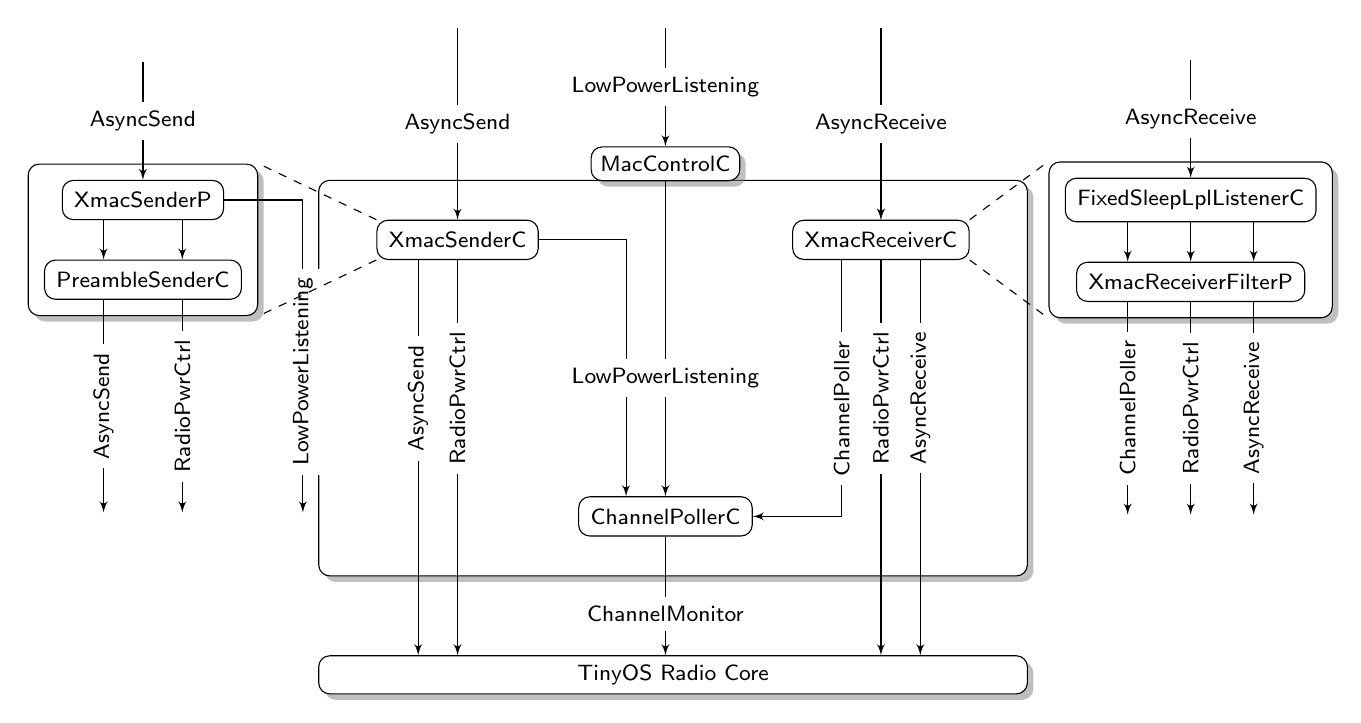
\begin{tikzpicture}
\tikzstyle{every node}=[font=\sffamily\footnotesize]

\node[layer, minimum width=9cm] (Core) { TinyOS Radio Core };

\node[layer, matrix, above=of Core, 
      column sep=5mm, row sep=30mm, inner sep=5mm,
      minimum width=9cm, nodes={reset, component}] (MacC) {
  \node (SenderC) {XmacSenderC}; & & \node (ReceiverC) {XmacReceiverC}; \\
  & \node (ChannelPollerC) {ChannelPollerC}; & \\
};

\node[layer, above=40mm of ChannelPollerC] (MacControlC) { MacControlC };

\node[layer, matrix, row sep=5mm, inner sep=2mm, nodes={reset, component}, 
  left=15mm of SenderC] (SenderDetail) {
  \node (XmacSenderP) { XmacSenderP }; \\
  \node (PreambleSenderC) { PreambleSenderC }; \\
};

\node[layer, matrix, row sep=5mm, inner sep=2mm, nodes={reset, component}, 
  right=10mm of ReceiverC] (ReceiverDetail) {
  \node (LplListenerC) { FixedSleepLplListenerC }; \\
  \node (RecvFilterP) { XmacReceiverFilterP }; \\
};


\coordinate[above=15mm of MacControlC] (Inputs) {};
\draw ([xshift=0mm] SenderC.south) coordinate (sout1) {};
\draw ([xshift=-5mm] SenderC.south) coordinate (sout2) {};

\draw ([xshift=0mm] ReceiverC.south) coordinate (rout1) {};
\draw ([xshift=5mm] ReceiverC.south) coordinate (rout2) {};

\coordinate[above=15mm of XmacSenderP] (xsin) {};
\coordinate[above=15mm of LplListenerC] (fslin) {};

\draw ([xshift=5mm] XmacSenderP.south) coordinate (xsout1) {};
\draw ([xshift=-5mm] XmacSenderP.south) coordinate (xsout2) {};
\draw ([xshift=10mm] XmacSenderP.east) coordinate (xsout3) {};

\draw ([xshift=8mm] LplListenerC.south) coordinate (fslout1) {};
\draw (LplListenerC.south) coordinate (fslout2) {};
\draw ([xshift=-8mm] LplListenerC.south) coordinate (fslout3) {};

\coordinate[below=27mm of PreambleSenderC] (psout) {};
\coordinate[below=27mm of RecvFilterP] (rcvout) {};

\draw ([xshift=-5mm] PreambleSenderC.south) coordinate (psout1) {};
\draw ([xshift=5mm] PreambleSenderC.south) coordinate (psout2) {};

\draw (RecvFilterP.south) coordinate (rcvout2) {};
\draw ([xshift=-8mm] RecvFilterP.south) coordinate (rcvout3) {};
\draw ([xshift=8mm] RecvFilterP.south) coordinate (rcvout1) {};


\draw[->] (Inputs) -- (MacControlC) node [midway, fill=white] { LowPowerListening };
\draw[->] (MacControlC) -- (MacControlC |- ChannelPollerC.north);
\draw[->] (SenderC) -| ([xshift=-5mm] ChannelPollerC.north);
%\draw[->] (ReceiverC) -| ([xshift=5mm] ChannelPollerC.north);
\draw[->] ([xshift=-5mm] ReceiverC.south) |- (ChannelPollerC.east) 
           node [pos=0.29, fill=white, rotate=90] { ChannelPoller };
\node[fill=white] at ([yshift=-25mm] MacControlC.south) (LPL) { LowPowerListening };
\draw[->] (ChannelPollerC.south) -- (MacControlC |- Core.north) 
           node [pos=0.65, fill=white] { ChannelMonitor };

\draw[->] (Inputs -| SenderC) -- (SenderC) node [midway, fill=white] { AsyncSend };
\draw[->] (sout1) -- (sout1 |- Core.north) node [pos=0.35, fill=white, rotate=90] { RadioPwrCtrl };
\draw[->] (sout2) -- (sout2 |- Core.north) node [pos=0.35, fill=white, rotate=90] { AsyncSend };

\draw[->] (xsin) -- (XmacSenderP) node [midway, fill=white] { AsyncSend };
\draw[->] (xsout1) -- (xsout1 |- PreambleSenderC.north);
\draw[->] (xsout2) -- (xsout2 |- PreambleSenderC.north);
\draw[->] (psout1) -- (psout1 |- psout) node [midway, fill=white, rotate=90] { AsyncSend };
\draw[->] (psout2) -- (psout2 |- psout) node [midway, fill=white, rotate=90] { RadioPwrCtrl };
\draw[->] (XmacSenderP.east) -- (xsout3) -- (xsout3 |- psout)
          node[pos=0.55, fill=white, rotate=90] { LowPowerListening };


\draw[->] (Inputs -| ReceiverC) -- (ReceiverC) node [midway, fill=white] { AsyncReceive };
\draw[->] (rout1) -- (rout1 |- Core.north) node [pos=0.35, fill=white, rotate=90] { RadioPwrCtrl };
\draw[->] (rout2) -- (rout2 |- Core.north) node [pos=0.35, fill=white, rotate=90] { AsyncReceive };

\draw[->] (fslin) -- (LplListenerC) node [midway, fill=white] { AsyncReceive };
\draw[->] (fslout1) -- (fslout1 |- RecvFilterP.north);
\draw[->] (fslout2) -- (fslout2 |- RecvFilterP.north);
\draw[->] (fslout3) -- (fslout3 |- RecvFilterP.north);
\draw[->] (rcvout1) -- (rcvout1 |- rcvout) node [midway, fill=white, rotate=90] { AsyncReceive };
\draw[->] (rcvout2) -- (rcvout2 |- rcvout) node [midway, fill=white, rotate=90] { RadioPwrCtrl };
\draw[->] (rcvout3) -- (rcvout3 |- rcvout) node [midway, fill=white, rotate=90] { ChannelPoller };

\draw[->] (Inputs -| ReceiverC) -- (ReceiverC) node [midway, fill=white] { AsyncReceive };

\draw[dashed] (SenderC.north west) -- (SenderDetail.north east);
\draw[dashed] (SenderC.south west) -- (SenderDetail.south east);

\draw[dashed] (ReceiverC.north east) -- (ReceiverDetail.north west);
\draw[dashed] (ReceiverC.south east) -- (ReceiverDetail.south west);

\end{tikzpicture}
%\end{document}

}

\Blindtext

% vim: set ft=tex

\chapter{Research Question or Problem Statement}
\label{chap:problemstatement}
Engineering theses tend to refer to a "problem" to be solved where other
disciplines talk in terms of a "question" to be answered. In either case, this
section has three main parts:

\begin{enumerate}
    \item A concise statement of the question that your thesis tackles
    \item Justification, by direct reference to section 3, that your question is previously unanswered
    \item Discussion of why it is worthwhile to answer this question.
\end{enumerate}

Item 2 above is where you analyze the information which you presented in
Section 3. For example, maybe your problem is to "develop a Zylon algorithm
capable of handling very large scale problems in reasonable time" (you would
further describe what you mean by "large scale" and "reasonable time" in the
problem statement). Now in your analysis of the state of the art you would
show how each class of current approaches fails (i.e. can handle only small
problems, or takes too much time). In the last part of this section you would
explain why having a large-scale fast Zylon algorithm is useful; e.g., by
describing applications where it can be used.

Since this is one of the sections that the readers are definitely looking for,
highlight it by using the word "problem" or "question" in the title: e.g.
"Research Question" or "Problem Statement", or maybe something more specific
such as "The Large-Scale Zylon Algorithm Problem." 

\section{A Note from the Template Author}
Again, this chapter might not be feasible for the scope of a master thesis.
Discuss with your advisor, if it is necessary, or if it might be better
integrated as the intoductory section of your contributions or as the last
section in the related work.

\section{Filler Text}
\blindtext
\blindtext
\blindenumerate
\blindtext
\blinddescription
\blindtext

% vim: set ft=tex

\chapter{Your Contribution}
\label{chap:contribution1}
This part of the thesis is much more free-form. It may have one or
several sections and subsections. But it all has only one purpose: to convince
the examiners that you answered the question or solved the problem that you
set for yourself in Section 4. So show what you did that is relevant to
answering the question or solving the problem: if there were blind alleys and
dead ends, do not include these, unless specifically relevant to the
demonstration that you answered the thesis question. 

\section{Filler Text}
\Blindtext



% vim: set ft=tex

\chapter{Your other Contribution}
\label{chap:contribution2}
This part of the thesis is much more free-form. It may have one or
several sections and subsections. But it all has only one purpose: to convince
the examiners that you answered the question or solved the problem that you
set for yourself in Section 4. So show what you did that is relevant to
answering the question or solving the problem: if there were blind alleys and
dead ends, do not include these, unless specifically relevant to the
demonstration that you answered the thesis question. 

\section{A Note from the Template Author}
You can span the text, describing your contribution over multiple chapters.
Again, discuss with your advisor whether this is feasible. But don't annoy
your advisor by asking him about how to structure your text. Think about what
you want to say, then create a structure, outline the content of that
structure and then present it to your advisor. 

\section{Filler Text}
\Blindtext

% vim: set ft=tex

\chapter{Conclusions}
\label{chap:conclusions}
You generally cover three things in the Conclusions section, and each of these
usually merits a separate subsection:

\begin{enumerate}
    \item Conclusions
    \item Summary of Contributions
    \item Future Research
\end{enumerate}

Conclusions are not a rambling summary of the thesis: they are short, concise
statements of the inferences that you have made because of your work. It helps
to organize these as short numbered paragraphs, ordered from most to least
important. All conclusions should be directly related to the research question
stated in Section 4. Examples:

\begin{enumerate}
    \item The problem stated in Section 4 has been solved: as shown in Sections ? to
    ??, an algorithm capable of handling large-scale Zylon problems in reasonable
    time has been developed.
    \item The principal mechanism needed in the improved Zylon algorithm is the Grooty mechanism.
    \item Etc.
\end{enumerate}

The Summary of Contributions will be much sought and carefully read by the
examiners. Here you list the contributions of new knowledge that your thesis
makes. Of course, the thesis itself must substantiate any claims made here.
There is often some overlap with the Conclusions, but that's okay. Concise
numbered paragraphs are again best. Organize from most to least important.
Examples:

\begin{enumerate}
    \item Developed a much quicker algorithm for large-scale Zylon problems.
    \item Demonstrated the first use of the Grooty mechanism for Zylon calculations.
    \item Etc.
\end{enumerate}

The Future Research subsection is included so that researchers picking up this
work in future have the benefit of the ideas that you generated while you were
working on the project. Again, concise numbered paragraphs are usually best. 

% vim: set ft=tex


\appendix
\part*{\appendixname}
\chapter{What goes in the appendices}
\label{app:a}
Any material which impedes the smooth development
of your presentation, but which is important to justify the results of a
thesis. Generally it is material that is of too nitty-gritty a level of detail
for inclusion in the main body of the thesis, but which should be available
for perusal by the examiners to convince them sufficiently. Examples include
program listings, immense tables of data, lengthy mathematical proofs or
derivations, etc. 

\section{Filler Text}
\Blindtext




% vim: set ft=tex

\chapter{Further remarks by Prof. Chinneck}
\label{app:b}
This appendix contains some remarks which followed the skeletal outline in the
original article by Prof. Chinneck. I needed to replace several things to make
them work with this template.

\section{Comments on the Thesis Skeleton}
Again, the thesis is a formal document designed to address the examiner's two
main questions. Chapter \ref{chap:relatedwork} and \ref{chap:problemstatement}
show that you have chosen a good problem, and Chapters
\ref{chap:contribution1} and \ref{chap:contribution2} show that you solved it.
Chapters \ref{chap:introduction} and \ref{chap:background} lead the reader
into the problem, and Chapter \ref{chap:conclusions} highlights the main
knowledge generated by the whole exercise.

Note also that everything that others did is carefully separated from
everything that you did. Knowing who did what is important to the examiners.
Section 4, the problem statement, is the obvious dividing line. That's the
main reason for putting it in the middle in this formal document.

\section{Getting Started}
The best way to get started on your thesis is to prepare an extended outline.
You begin by making up the Table of Contents, listing each section and
subsection that you propose to include. For each section and subsection, write
a brief point-form description of the contents of that section. The entire
outline might be 2 to 5 pages long. Now you and your thesis supervisor should
carefully review this outline: is there unnecessary material (i.e. not
directly related to the problem statement)? Then remove. Is there missing
material? Then add. It is much less painful and more time-efficient to make
such decisions early, during the outline phase, rather than after you've
already done a lot of writing which has to be thrown away.  


\section{How Long Does it Take to Write a Thesis?}
Longer than you think. Even after the research itself is all done -- models
built, calculations complete -- it is wise to allow at least one complete term
for writing the thesis. It's not the physical act of typing that takes so
long, it's the fact that writing the thesis requires the complete organization
of your arguments and results. It's during this formalization of your results
into a well-organized thesis document capable of withstanding the scrutiny of
expert examiners that you discover weaknesses. It's fixing those weaknesses
that takes time.

This is also probably the first time that your supervisor has seen the formal
expression of concepts that may have been approved previously in an informal
manner. Now is when you discover any misunderstandings or shortcomings in the
informal agreements. It takes time to fix these. Students for whom english is
not the mother tongue may have difficulty in getting ideas across, so that
numerous revisions are required. And, truth be known, supervisors are
sometimes not quick at reviewing and returning drafts.

\subsection*{Bottom line:} leave yourself enough time. A rush job has painful consequences
at the defence\footnote{Template Author's note: in case of a master thesis
this is not a defence but only a 'final presentation'. In any way, you need to
present your work and you might get awkward questions, based on the quality of
your work.}

\section{Tips}

Always keep the reader's backgrounds in mind. Who is your audience? How much
can you reasonably expect them to know about the subject before picking up
your thesis? Usually they are pretty knowledgeable about the general problem,
but they haven't been intimately involved with the details over the last
couple of years like you have: spell difficult new concepts out clearly. It
sometimes helps to mentally picture a real person that you know who has the
appropriate background, and to imagine that you are explaining your ideas
directly to that person.

Don't make the readers work too hard! This is fundamentally important. You
know what few questions the examiners need answers for (see above). Choose
section titles and wordings to clearly give them this information. The harder
they have to work to ferret out your problem, your defence of the problem,
your answer to the problem, your conclusions and contributions, the worse mood
they will be in, and the more likely that your thesis will need major
revisions.

A corollary of the above: it's impossible to be too clear! Spell things out
carefully, highlight important parts by appropriate titles etc. There's a huge
amount of information in a thesis: make sure you direct the readers to the
answers to the important questions.

Remember that a thesis is not a story: it usually doesn't follow the
chronology of things that you tried. It's a formal document designed to answer
only a few major questions.

Avoid using phrases like "Clearly, this is the case..." or "Obviously, it
follows that ..."; these imply that, if the readers don't understand, then
they must be stupid. They might not have understood because you explained it
poorly.

Avoid red flags, claims (like "software is the most important part of a
computer system") that are really only your personal opinion and not
substantiated by the literature or the solution you have presented. Examiners
like to pick on sentences like that and ask questions like, "Can you
demonstrate that software is the most important part of a computer system?"

\section{A Note on Computer Programs and Other Prototypes}
The purpose of your thesis is to clearly document an original contribution to
knowledge. You may develop computer programs, prototypes, or other tools as a
means of proving your points, but remember, the thesis is not about the tool,
it is about the contribution to knowledge. Tools such as computer programs are
fine and useful products, but you can't get an advanced degree just for the
tool. You must use the tool to demonstrate that you have made an original
contribution to knowledge; e.g., through its use, or ideas it embodies.

\section{Master's vs. PhD Thesis}
There are different expectations for Master's theses and for Doctoral theses.
This difference is not in format but in the significance and level of
discovery as evidenced by the problem to be solved and the summary of
contributions; a Doctoral thesis necessarily requires a more difficult problem
to be solved, and consequently more substantial contributions.

The contribution to knowledge of a Master's thesis can be in the nature of an
incremental improvement in an area of knowledge, or the application of known
techniques in a new area. The Ph.D. must be a substantial and innovative
contribution to knowledge.  

% vim: set ft=tex

%\chapter{Used Acronyms}
    \begin{acronym}
\end{acronym}
 % See acrodb.tex for info
\chapter{Used Acronyms}
\begin{acronym}
% Information on how to use the acronyms can be found here: http://www.mackichan.com/index.html?techtalk/456.htm~mainFrame
        \acro{API}{application programming interface}
        \acro{ANF}[A\& F]{Amplify \& Forward}
	\acro{ACK}{acknowledgment}
	\acro{ARP}{address resolution protocol}
        \acro{BLR}{Beaconless Routing}
	\acro{BPSK}{binary phase shift keying}
	\acro{CA}{collision avoidance}
	\acro{CCA}{clear channel assessment}
	\acro{CI}{confidence interval}
	\acro{CL}{confidence level}
        \acro{CNF}[C\& F]{Compress \& Forward}
        \acro{CPU}{Central Processing Unit}
	\acro{cRTS}{cooperative request-to-send}
        \acro{CSMA}{carrier sense multiple access}
        \acro{CSMA/CA}{\ac{CSMA} with \acf{CA}}
	\acro{CTS}{clear-to-send}
        \acro{CTP}{Collection Tree Protocol}
	\acro{CVS}{concurrent versioning system}
	\acro{DCF}{distributed coordination function}
	\acro{DIFS}{\acs{DCF} inter-frame spacing}
	\acro{DMA}{direct memory access}
        \acro{DNF}[D\& F]{Decode \& Forward}
	\acro{DSP}{digital signal processor}
	\acro{EIFS}{extended inter-frame spacing}
        \acro{EMA}{exponential moving average}
        \acro{ETX}{expected transmissions}
        \acro{ExOR}{Extremely Opportunistic Routing}
	\acro{FCS}{frame checksum}
        \acro{FER}{frame error rate}
	\acro{FPGA}{field programmable gate array}
	\acro{FTP}{file transfer protocol}
        \acro{GeRaF}{Geographic Random Forwarding}
	\acro{GP}{goodput}
	\acro{GPS}{Global Positioning System}
	\acro{HF}{high frequency}
	\acro{IEEE}{Institute of Electrical and Electronics Engineers}
	\acro{IHP}{Innovations for High Performance Microelectronics}
	\acro{IP}{Internet Protocol}
	\acro{ISR}{interrupt service routine}
	\acro{JTAG}{Joint Test Action Group}
	\acro{LAN}{local area network}
	\acro{LED}{light emitting diode}
	\acro{LOS}{line-of-sight}
	\acro{LSB}{least significant bit} 
	\acro{MAC}{medium access control}
        \acro{MLA}{MAC Layer Architecture}
        \acro{MLME}{MAC layer management entity}
	\acro{MS}{milestone}
	\acro{MSC}{message sequence chart}
        \acro{MTU}{maximum transmission unit}
	\acro{NAV}{network allocation vector}
        \acro{NesC}{Networked embedded systems C}
	\acro{NIF}{noise-and-interference floor}
	\acro{NLOS}{non-line-of-sight}
	\acro{OFDM}{orthogonal frequency-division multiplexing}
        \acro{ORM}{object-relational mapping}
	\acro{PER}{packet error rate}
	\acro{PG1}{Project Group Mobile Communications 1}
	\acro{PG2}{Project Group Mobile Communications 2}
	\acro{PHY}{physical}
        \acro{RBS}{referece brodcast synchronization scheme}
	\acro{RF}{radio frontend}
	\acro{RSSI}{received signal strength indicator}
	\acro{RTS}{request-to-send}
        \acro{SDF}{selection decode \& forward}
	\acro{SDL}{Specification and Description Language}
	\acro{SDR}{software-defined radio}
	\acro{SIFS}{short inter-frame spacing}
	\acro{SINR}{signal-to-interference-and-noise ratio}
	\acro{SORBAS}{Signalion Software Radio Based Prototyping System}
	\acro{SSH}{secure shell}
	\acro{SSID}{service set identifier}
	\acro{Sterm}{\acs{SORBAS} terminal}
	\acro{TX}{transmission}
        \acro{TDMA}{Time Division Multiple Access}
        \acro{TEP}{TinyOS Enhancement Proposal}
	\acro{UDP}{User Datagram Protocol}
	\acro{USB}{Universal Serial Bus}
        \acro{UPMA}{Unified radio Power Management Architecture}
	\acro{VisualDSP}{Visual Digital Signal Processor}
	\acro{VMware}{VMware Virtualization Software}
	\acro{VoIP}{voice over \acs{IP}}
	\acro{WinTerm}{SORBAS Windows Terminal}
	\acro{WLAN}{wireless \acs{LAN}}
        \acro{WMA}{weighted moving average}
        \acro{WSN}{wireless sensor network}
\end{acronym}

% vim: set ft=latex


% Bibliography
\bibliographystyle{plain}
\bibliography{thesis}
%
\backmatter
\chapter*{Erklärung der Urheberschaft}
\vfill
Hiermit versichere ich, dass ich die vorliegende Diplomarbeit ohne Hilfe
Dritter und ohne Benutzung anderer als der angegebenen Quellen und Hilfsmittel
angefertigt habe. Wörtlich oder dem Sinn nach aus anderen Werken entnommene
Stellen sind unter Angabe der Quellen kenntlich gemacht. Diese Arbeit hat in
gleicher oder ähnlicher Form noch keiner Prüfungsbehörde vorgelegen.

\par\vfill\vfill\noindent
\hrulefill\hfill\hrulefill\\
Ort, Datum  \hfill Unterschrift\\


\newpage
\thispagestyle{empty}

% vim: set ft=tex

%
\end{document}
%EOF
% vim: set ft=tex
